\documentclass[1p]{elsarticle_modified}
%\bibliographystyle{elsarticle-num}

%\usepackage[colorlinks]{hyperref}
%\usepackage{abbrmath_seonhwa} %\Abb, \Ascr, \Acal ,\Abf, \Afrak
\usepackage{amsfonts}
\usepackage{amssymb}
\usepackage{amsmath}
\usepackage{amsthm}
\usepackage{scalefnt}
\usepackage{amsbsy}
\usepackage{kotex}
\usepackage{caption}
\usepackage{subfig}
\usepackage{color}
\usepackage{graphicx}
\usepackage{xcolor} %% white, black, red, green, blue, cyan, magenta, yellow
\usepackage{float}
\usepackage{setspace}
\usepackage{hyperref}

\usepackage{tikz}
\usetikzlibrary{arrows}

\usepackage{multirow}
\usepackage{array} % fixed length table
\usepackage{hhline}

%%%%%%%%%%%%%%%%%%%%%
\makeatletter
\renewcommand*\env@matrix[1][\arraystretch]{%
	\edef\arraystretch{#1}%
	\hskip -\arraycolsep
	\let\@ifnextchar\new@ifnextchar
	\array{*\c@MaxMatrixCols c}}
\makeatother %https://tex.stackexchange.com/questions/14071/how-can-i-increase-the-line-spacing-in-a-matrix
%%%%%%%%%%%%%%%

\usepackage[normalem]{ulem}

\newcommand{\msout}[1]{\ifmmode\text{\sout{\ensuremath{#1}}}\else\sout{#1}\fi}
%SOURCE: \msout is \stkout macro in https://tex.stackexchange.com/questions/20609/strikeout-in-math-mode

\newcommand{\cancel}[1]{
	\ifmmode
	{\color{red}\msout{#1}}
	\else
	{\color{red}\sout{#1}}
	\fi
}

\newcommand{\add}[1]{
	{\color{blue}\uwave{#1}}
}

\newcommand{\replace}[2]{
	\ifmmode
	{\color{red}\msout{#1}}{\color{blue}\uwave{#2}}
	\else
	{\color{red}\sout{#1}}{\color{blue}\uwave{#2}}
	\fi
}

\newcommand{\Sol}{\mathcal{S}} %segment
\newcommand{\D}{D} %diagram
\newcommand{\A}{\mathcal{A}} %arc


%%%%%%%%%%%%%%%%%%%%%%%%%%%%%5 test

\def\sl{\operatorname{\textup{SL}}(2,\Cbb)}
\def\psl{\operatorname{\textup{PSL}}(2,\Cbb)}
\def\quan{\mkern 1mu \triangleright \mkern 1mu}

\theoremstyle{definition}
\newtheorem{thm}{Theorem}[section]
\newtheorem{prop}[thm]{Proposition}
\newtheorem{lem}[thm]{Lemma}
\newtheorem{ques}[thm]{Question}
\newtheorem{cor}[thm]{Corollary}
\newtheorem{defn}[thm]{Definition}
\newtheorem{exam}[thm]{Example}
\newtheorem{rmk}[thm]{Remark}
\newtheorem{alg}[thm]{Algorithm}

\newcommand{\I}{\sqrt{-1}}
\begin{document}

%\begin{frontmatter}
%
%\title{Boundary parabolic representations of knots up to 8 crossings}
%
%%% Group authors per affiliation:
%\author{Yunhi Cho} 
%\address{Department of Mathematics, University of Seoul, Seoul, Korea}
%\ead{yhcho@uos.ac.kr}
%
%
%\author{Seonhwa Kim} %\fnref{s_kim}}
%\address{Center for Geometry and Physics, Institute for Basic Science, Pohang, 37673, Korea}
%\ead{ryeona17@ibs.re.kr}
%
%\author{Hyuk Kim}
%\address{Department of Mathematical Sciences, Seoul National University, Seoul 08826, Korea}
%\ead{hyukkim@snu.ac.kr}
%
%\author{Seokbeom Yoon}
%\address{Department of Mathematical Sciences, Seoul National University, Seoul, 08826,  Korea}
%\ead{sbyoon15@snu.ac.kr}
%
%\begin{abstract}
%We find all boundary parabolic representation of knots up to 8 crossings.
%
%\end{abstract}
%\begin{keyword}
%    \MSC[2010] 57M25 
%\end{keyword}
%
%\end{frontmatter}

%\linenumbers
%\tableofcontents
%
\newcommand\colored[1]{\textcolor{white}{\rule[-0.35ex]{0.8em}{1.4ex}}\kern-0.8em\color{red} #1}%
%\newcommand\colored[1]{\textcolor{white}{ #1}\kern-2.17ex	\textcolor{white}{ #1}\kern-1.81ex	\textcolor{white}{ #1}\kern-2.15ex\color{red}#1	}

{\Large $\underline{11a_{40}~(K11a_{40})}$}

\setlength{\tabcolsep}{10pt}
\renewcommand{\arraystretch}{1.6}
\vspace{1cm}\begin{tabular}{m{100pt}>{\centering\arraybackslash}m{274pt}}
\multirow{5}{120pt}{
	\centering
	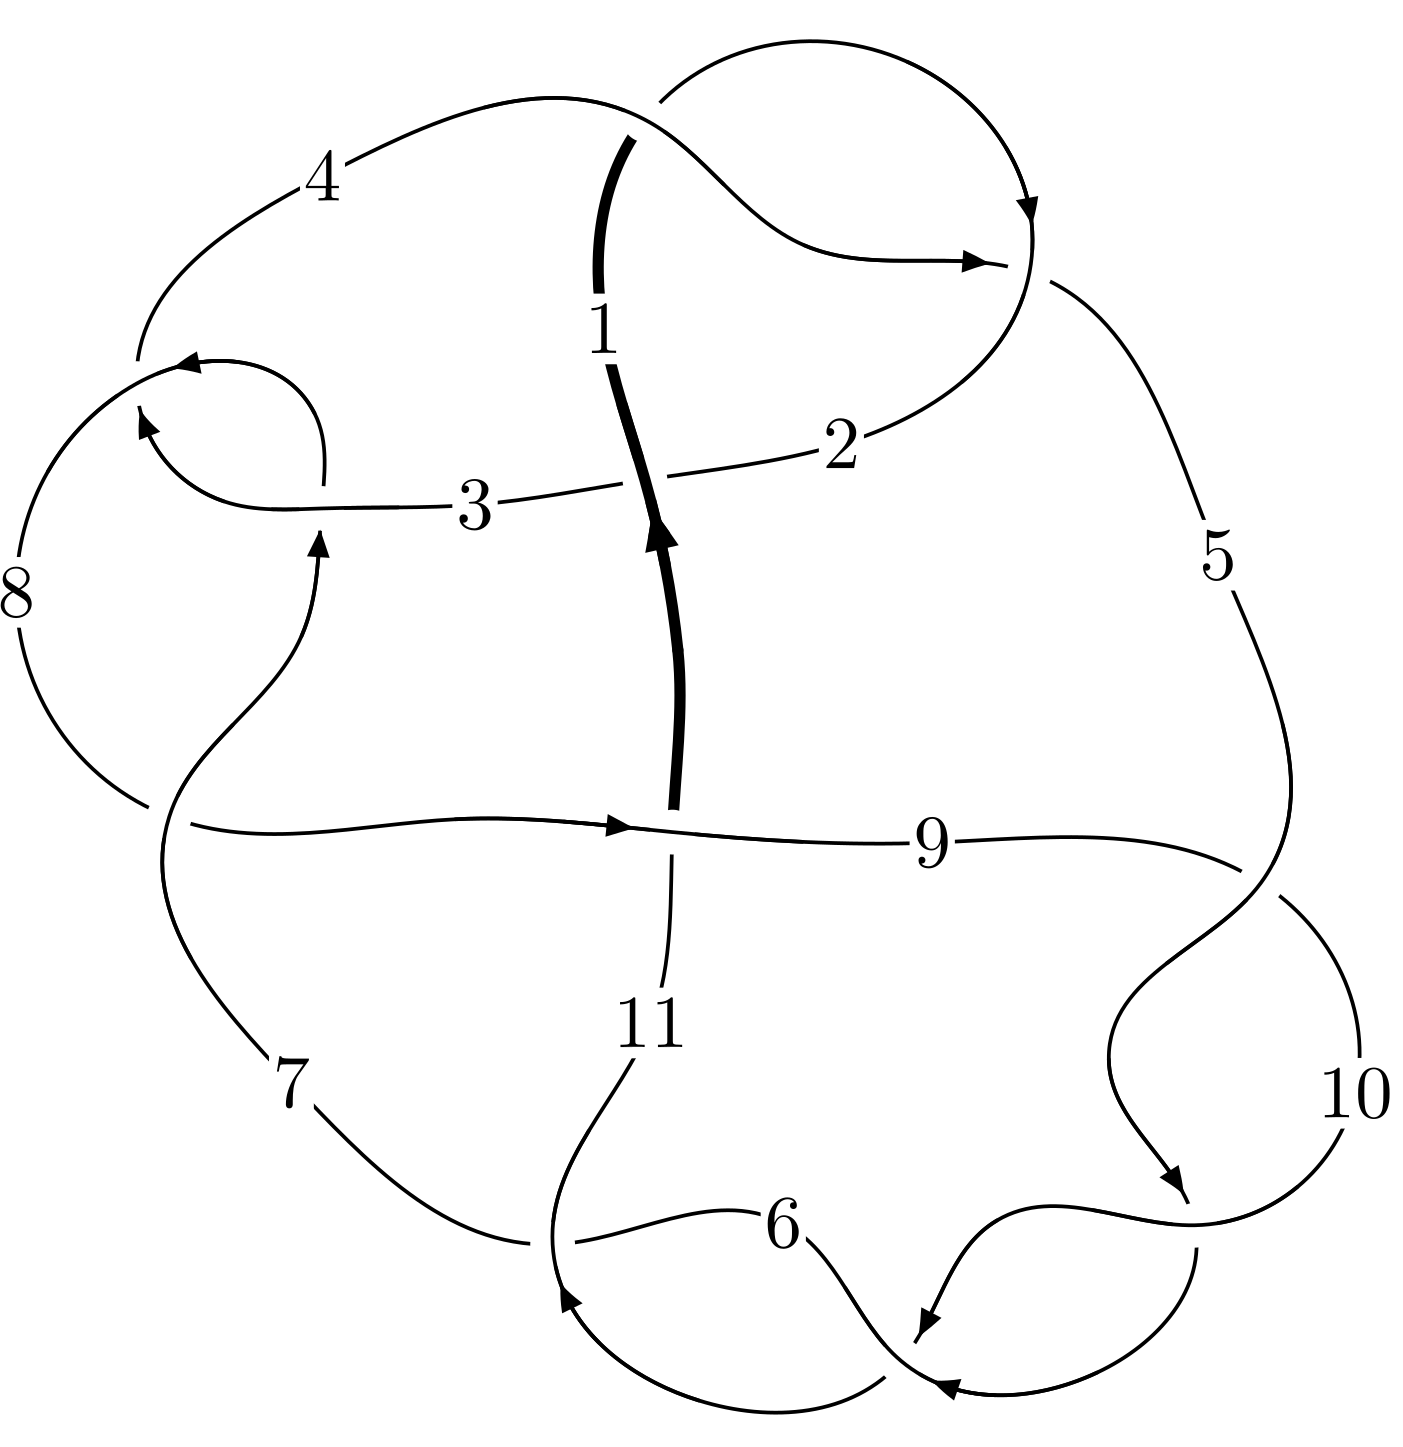
\includegraphics[width=112pt]{../../../GIT/diagram.site/Diagrams/png/289_11a_40.png}\\
\ \ \ A knot diagram\footnotemark}&
\allowdisplaybreaks
\textbf{Linearized knot diagam} \\
\cline{2-2}
 &
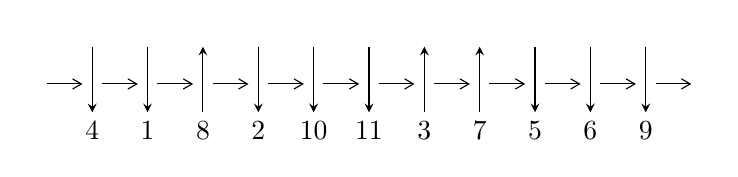
\begin{tikzpicture}[x=20pt, y=17pt]
	% nodes
	\node (C0) at (0, 0) {};
	\node (C1) at (1, 0) {};
	\node (C1U) at (1, +1) {};
	\node (C1D) at (1, -1) {4};

	\node (C2) at (2, 0) {};
	\node (C2U) at (2, +1) {};
	\node (C2D) at (2, -1) {1};

	\node (C3) at (3, 0) {};
	\node (C3U) at (3, +1) {};
	\node (C3D) at (3, -1) {8};

	\node (C4) at (4, 0) {};
	\node (C4U) at (4, +1) {};
	\node (C4D) at (4, -1) {2};

	\node (C5) at (5, 0) {};
	\node (C5U) at (5, +1) {};
	\node (C5D) at (5, -1) {10};

	\node (C6) at (6, 0) {};
	\node (C6U) at (6, +1) {};
	\node (C6D) at (6, -1) {11};

	\node (C7) at (7, 0) {};
	\node (C7U) at (7, +1) {};
	\node (C7D) at (7, -1) {3};

	\node (C8) at (8, 0) {};
	\node (C8U) at (8, +1) {};
	\node (C8D) at (8, -1) {7};

	\node (C9) at (9, 0) {};
	\node (C9U) at (9, +1) {};
	\node (C9D) at (9, -1) {5};

	\node (C10) at (10, 0) {};
	\node (C10U) at (10, +1) {};
	\node (C10D) at (10, -1) {6};

	\node (C11) at (11, 0) {};
	\node (C11U) at (11, +1) {};
	\node (C11D) at (11, -1) {9};
	\node (C12) at (12, 0) {};

	% arrows
	\draw[->,>={angle 60}]
	(C0) edge (C1) (C1) edge (C2) (C2) edge (C3) (C3) edge (C4) (C4) edge (C5) (C5) edge (C6) (C6) edge (C7) (C7) edge (C8) (C8) edge (C9) (C9) edge (C10) (C10) edge (C11) (C11) edge (C12) ;	\draw[->,>=stealth]
	(C1U) edge (C1D) (C2U) edge (C2D) (C3D) edge (C3U) (C4U) edge (C4D) (C5U) edge (C5D) (C6U) edge (C6D) (C7D) edge (C7U) (C8D) edge (C8U) (C9U) edge (C9D) (C10U) edge (C10D) (C11U) edge (C11D) ;
	\end{tikzpicture} \\
\hhline{~~} \\& 
\textbf{Solving Sequence} \\ \cline{2-2} 
 &
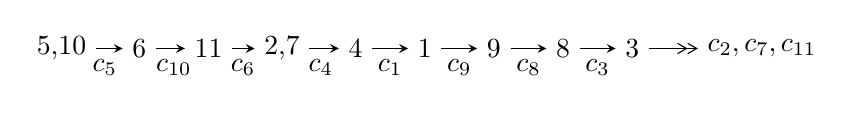
\begin{tikzpicture}[x=25pt, y=7pt]
	% node
	\node (A0) at (-1/8, 0) {5,10};
	\node (A1) at (1, 0) {6};
	\node (A2) at (2, 0) {11};
	\node (A3) at (49/16, 0) {2,7};
	\node (A4) at (33/8, 0) {4};
	\node (A5) at (41/8, 0) {1};
	\node (A6) at (49/8, 0) {9};
	\node (A7) at (57/8, 0) {8};
	\node (A8) at (65/8, 0) {3};
	\node (C1) at (1/2, -1) {$c_{5}$};
	\node (C2) at (3/2, -1) {$c_{10}$};
	\node (C3) at (5/2, -1) {$c_{6}$};
	\node (C4) at (29/8, -1) {$c_{4}$};
	\node (C5) at (37/8, -1) {$c_{1}$};
	\node (C6) at (45/8, -1) {$c_{9}$};
	\node (C7) at (53/8, -1) {$c_{8}$};
	\node (C8) at (61/8, -1) {$c_{3}$};
	\node (A9) at (10, 0) {$c_{2},c_{7},c_{11}$};

	% edge
	\draw[->,>=stealth]	
	(A0) edge (A1) (A1) edge (A2) (A2) edge (A3) (A3) edge (A4) (A4) edge (A5) (A5) edge (A6) (A6) edge (A7) (A7) edge (A8) ;
	\draw[->>,>={angle 60}]	
	(A8) edge (A9);
\end{tikzpicture} \\ 

\end{tabular} \\

\footnotetext{
The image of knot diagram is generated by the software ``\textbf{Draw programme}" developed by Andrew Bartholomew(\url{http://www.layer8.co.uk/maths/draw/index.htm\#Running-draw}), where we modified some parts for our purpose(\url{https://github.com/CATsTAILs/LinksPainter}).
}\phantom \\ \newline 
\centering \textbf{Ideals for irreducible components\footnotemark of $X_{\text{par}}$} 
 
\begin{align*}
I^u_{1}&=\langle 
- u^{45}- u^{44}+\cdots+b+u,\;- u^{45}- u^{44}+\cdots+a+1,\;u^{46}+2 u^{45}+\cdots- u+1\rangle \\
I^u_{2}&=\langle 
b+1,\;a+2,\;u^2+u-1\rangle \\
\\
\end{align*}
\raggedright * 2 irreducible components of $\dim_{\mathbb{C}}=0$, with total 48 representations.\\
\footnotetext{All coefficients of polynomials are rational numbers. But the coefficients are sometimes approximated in decimal forms when there is not enough margin.}
\newpage
\renewcommand{\arraystretch}{1}
\centering \section*{I. $I^u_{1}= \langle - u^{45}- u^{44}+\cdots+b+u,\;- u^{45}- u^{44}+\cdots+a+1,\;u^{46}+2 u^{45}+\cdots- u+1 \rangle$}
\flushleft \textbf{(i) Arc colorings}\\
\begin{tabular}{m{7pt} m{180pt} m{7pt} m{180pt} }
\flushright $a_{5}=$&$\begin{pmatrix}1\\0\end{pmatrix}$ \\
\flushright $a_{10}=$&$\begin{pmatrix}0\\u\end{pmatrix}$ \\
\flushright $a_{6}=$&$\begin{pmatrix}1\\u^2\end{pmatrix}$ \\
\flushright $a_{11}=$&$\begin{pmatrix}- u\\- u^3+u\end{pmatrix}$ \\
\flushright $a_{2}=$&$\begin{pmatrix}u^{45}+u^{44}+\cdots-3 u-1\\u^{45}+u^{44}+\cdots-2 u^2- u\end{pmatrix}$ \\
\flushright $a_{7}=$&$\begin{pmatrix}- u^2+1\\- u^4+2 u^2\end{pmatrix}$ \\
\flushright $a_{4}=$&$\begin{pmatrix}2 u^{45}+2 u^{44}+\cdots-6 u^3-3 u\\u^{45}+u^{44}+\cdots-2 u^2-2 u\end{pmatrix}$ \\
\flushright $a_{1}=$&$\begin{pmatrix}u^5-2 u^3- u\\u^5-3 u^3+u\end{pmatrix}$ \\
\flushright $a_{9}=$&$\begin{pmatrix}u\\u\end{pmatrix}$ \\
\flushright $a_{8}=$&$\begin{pmatrix}u^7-4 u^5+4 u^3\\u^9-5 u^7+7 u^5-2 u^3+u\end{pmatrix}$ \\
\flushright $a_{3}=$&$\begin{pmatrix}- u^{38}+21 u^{36}+\cdots-2 u-1\\u^{45}+u^{44}+\cdots-3 u^2- u\end{pmatrix}$\\ \flushright $a_{3}=$&$\begin{pmatrix}- u^{38}+21 u^{36}+\cdots-2 u-1\\u^{45}+u^{44}+\cdots-3 u^2- u\end{pmatrix}$\\&\end{tabular}
\flushleft \textbf{(ii) Obstruction class $= -1$}\\~\\
\flushleft \textbf{(iii) Cusp Shapes $= 4 u^{45}+u^{44}+\cdots+8 u-1$}\\~\\
\newpage\renewcommand{\arraystretch}{1}
\flushleft \textbf{(iv) u-Polynomials at the component}\newline \\
\begin{tabular}{m{50pt}|m{274pt}}
Crossings & \hspace{64pt}u-Polynomials at each crossing \\
\hline $$\begin{aligned}c_{1},c_{4}\end{aligned}$$&$\begin{aligned}
&u^{46}-3 u^{45}+\cdots-4 u+1
\end{aligned}$\\
\hline $$\begin{aligned}c_{2}\end{aligned}$$&$\begin{aligned}
&u^{46}+25 u^{45}+\cdots+4 u+1
\end{aligned}$\\
\hline $$\begin{aligned}c_{3},c_{7}\end{aligned}$$&$\begin{aligned}
&u^{46}+u^{45}+\cdots+8 u+4
\end{aligned}$\\
\hline $$\begin{aligned}c_{5},c_{6},c_{9}\\c_{10}\end{aligned}$$&$\begin{aligned}
&u^{46}+2 u^{45}+\cdots- u+1
\end{aligned}$\\
\hline $$\begin{aligned}c_{8}\end{aligned}$$&$\begin{aligned}
&u^{46}-15 u^{45}+\cdots-232 u+16
\end{aligned}$\\
\hline $$\begin{aligned}c_{11}\end{aligned}$$&$\begin{aligned}
&u^{46}-14 u^{45}+\cdots-885 u+207
\end{aligned}$\\
\hline
\end{tabular}\\~\\
\newpage\renewcommand{\arraystretch}{1}
\flushleft \textbf{(v) Riley Polynomials at the component}\newline \\
\begin{tabular}{m{50pt}|m{274pt}}
Crossings & \hspace{64pt}Riley Polynomials at each crossing \\
\hline $$\begin{aligned}c_{1},c_{4}\end{aligned}$$&$\begin{aligned}
&y^{46}-25 y^{45}+\cdots-4 y+1
\end{aligned}$\\
\hline $$\begin{aligned}c_{2}\end{aligned}$$&$\begin{aligned}
&y^{46}-5 y^{45}+\cdots-44 y+1
\end{aligned}$\\
\hline $$\begin{aligned}c_{3},c_{7}\end{aligned}$$&$\begin{aligned}
&y^{46}-15 y^{45}+\cdots-232 y+16
\end{aligned}$\\
\hline $$\begin{aligned}c_{5},c_{6},c_{9}\\c_{10}\end{aligned}$$&$\begin{aligned}
&y^{46}-54 y^{45}+\cdots-9 y+1
\end{aligned}$\\
\hline $$\begin{aligned}c_{8}\end{aligned}$$&$\begin{aligned}
&y^{46}+29 y^{45}+\cdots-9760 y+256
\end{aligned}$\\
\hline $$\begin{aligned}c_{11}\end{aligned}$$&$\begin{aligned}
&y^{46}-18 y^{45}+\cdots-704565 y+42849
\end{aligned}$\\
\hline
\end{tabular}\\~\\
\newpage\flushleft \textbf{(vi) Complex Volumes and Cusp Shapes}
$$\begin{array}{c|c|c}  
\text{Solutions to }I^u_{1}& \I (\text{vol} + \sqrt{-1}CS) & \text{Cusp shape}\\
 \hline 
\begin{aligned}
u &= -0.869521 + 0.344145 I \\
a &= \phantom{-}1.50416 + 0.73434 I \\
b &= \phantom{-}1.129120 + 0.456816 I\end{aligned}
 & -4.45409 - 3.41461 I & -10.48322 + 2.63232 I \\ \hline\begin{aligned}
u &= -0.869521 - 0.344145 I \\
a &= \phantom{-}1.50416 - 0.73434 I \\
b &= \phantom{-}1.129120 - 0.456816 I\end{aligned}
 & -4.45409 + 3.41461 I & -10.48322 - 2.63232 I \\ \hline\begin{aligned}
u &= \phantom{-}0.755545 + 0.498860 I \\
a &= \phantom{-}1.99178 - 1.61778 I \\
b &= \phantom{-}1.180690 + 0.538180 I\end{aligned}
 & -3.31037 - 10.45050 I & -8.69927 + 9.35917 I \\ \hline\begin{aligned}
u &= \phantom{-}0.755545 - 0.498860 I \\
a &= \phantom{-}1.99178 + 1.61778 I \\
b &= \phantom{-}1.180690 - 0.538180 I\end{aligned}
 & -3.31037 + 10.45050 I & -8.69927 - 9.35917 I \\ \hline\begin{aligned}
u &= \phantom{-}0.711638 + 0.469005 I \\
a &= -0.763674 - 0.318200 I \\
b &= \phantom{-}0.203438 - 0.815815 I\end{aligned}
 & -0.41848 - 5.45501 I & -5.35190 + 6.48052 I \\ \hline\begin{aligned}
u &= \phantom{-}0.711638 - 0.469005 I \\
a &= -0.763674 + 0.318200 I \\
b &= \phantom{-}0.203438 + 0.815815 I\end{aligned}
 & -0.41848 + 5.45501 I & -5.35190 - 6.48052 I \\ \hline\begin{aligned}
u &= -0.735390 + 0.424801 I \\
a &= -2.02595 - 2.04160 I \\
b &= -1.135150 + 0.447303 I\end{aligned}
 & -4.51433 + 4.40744 I & -10.64051 - 5.57891 I \\ \hline\begin{aligned}
u &= -0.735390 - 0.424801 I \\
a &= -2.02595 + 2.04160 I \\
b &= -1.135150 - 0.447303 I\end{aligned}
 & -4.51433 - 4.40744 I & -10.64051 + 5.57891 I \\ \hline\begin{aligned}
u &= \phantom{-}0.745322 + 0.383218 I \\
a &= -1.65094 + 0.77106 I \\
b &= -1.213930 + 0.324837 I\end{aligned}
 & -4.79298 - 1.73712 I & -11.07336 + 4.61384 I \\ \hline\begin{aligned}
u &= \phantom{-}0.745322 - 0.383218 I \\
a &= -1.65094 - 0.77106 I \\
b &= -1.213930 - 0.324837 I\end{aligned}
 & -4.79298 + 1.73712 I & -11.07336 - 4.61384 I\\
 \hline 
 \end{array}$$\newpage$$\begin{array}{c|c|c}  
\text{Solutions to }I^u_{1}& \I (\text{vol} + \sqrt{-1}CS) & \text{Cusp shape}\\
 \hline 
\begin{aligned}
u &= -0.789174\phantom{ +0.000000I} \\
a &= \phantom{-}1.29622\phantom{ +0.000000I} \\
b &= \phantom{-}0.519026\phantom{ +0.000000I}\end{aligned}
 & -1.45882\phantom{ +0.000000I} & -5.44130\phantom{ +0.000000I} \\ \hline\begin{aligned}
u &= -0.727976 + 0.286689 I \\
a &= \phantom{-}0.947922 - 0.230896 I \\
b &= -0.010899 - 0.557387 I\end{aligned}
 & -1.56660 + 0.49532 I & -7.68115 - 1.36018 I \\ \hline\begin{aligned}
u &= -0.727976 - 0.286689 I \\
a &= \phantom{-}0.947922 + 0.230896 I \\
b &= -0.010899 + 0.557387 I\end{aligned}
 & -1.56660 - 0.49532 I & -7.68115 + 1.36018 I \\ \hline\begin{aligned}
u &= \phantom{-}0.508676 + 0.507354 I \\
a &= \phantom{-}0.77267 - 1.48119 I \\
b &= \phantom{-}0.827592 + 0.600489 I\end{aligned}
 & \phantom{-}2.79032 - 4.13635 I & -1.98154 + 7.56914 I \\ \hline\begin{aligned}
u &= \phantom{-}0.508676 - 0.507354 I \\
a &= \phantom{-}0.77267 + 1.48119 I \\
b &= \phantom{-}0.827592 - 0.600489 I\end{aligned}
 & \phantom{-}2.79032 + 4.13635 I & -1.98154 - 7.56914 I \\ \hline\begin{aligned}
u &= \phantom{-}0.393201 + 0.514206 I \\
a &= -0.490341 + 0.227249 I \\
b &= \phantom{-}0.712026 - 0.604892 I\end{aligned}
 & \phantom{-}3.12084 + 0.58749 I & -0.262566 + 0.327262 I \\ \hline\begin{aligned}
u &= \phantom{-}0.393201 - 0.514206 I \\
a &= -0.490341 - 0.227249 I \\
b &= \phantom{-}0.712026 + 0.604892 I\end{aligned}
 & \phantom{-}3.12084 - 0.58749 I & -0.262566 - 0.327262 I \\ \hline\begin{aligned}
u &= \phantom{-}0.109343 + 0.629269 I \\
a &= \phantom{-}0.371133 + 0.758125 I \\
b &= \phantom{-}1.143360 - 0.519855 I\end{aligned}
 & -1.40155 + 6.64307 I & -5.04471 - 5.15805 I \\ \hline\begin{aligned}
u &= \phantom{-}0.109343 - 0.629269 I \\
a &= \phantom{-}0.371133 - 0.758125 I \\
b &= \phantom{-}1.143360 + 0.519855 I\end{aligned}
 & -1.40155 - 6.64307 I & -5.04471 + 5.15805 I \\ \hline\begin{aligned}
u &= \phantom{-}0.147821 + 0.548345 I \\
a &= \phantom{-}0.106291 - 0.656538 I \\
b &= \phantom{-}0.241472 + 0.712682 I\end{aligned}
 & \phantom{-}1.22062 + 1.95597 I & -0.98131 - 1.36818 I\\
 \hline 
 \end{array}$$\newpage$$\begin{array}{c|c|c}  
\text{Solutions to }I^u_{1}& \I (\text{vol} + \sqrt{-1}CS) & \text{Cusp shape}\\
 \hline 
\begin{aligned}
u &= \phantom{-}0.147821 - 0.548345 I \\
a &= \phantom{-}0.106291 + 0.656538 I \\
b &= \phantom{-}0.241472 - 0.712682 I\end{aligned}
 & \phantom{-}1.22062 - 1.95597 I & -0.98131 + 1.36818 I \\ \hline\begin{aligned}
u &= -1.48057 + 0.06828 I \\
a &= \phantom{-}0.242649 + 0.138771 I \\
b &= \phantom{-}0.572969 + 0.701430 I\end{aligned}
 & -2.87293 + 1.27541 I & \phantom{-0.000000 } 0 \\ \hline\begin{aligned}
u &= -1.48057 - 0.06828 I \\
a &= \phantom{-}0.242649 - 0.138771 I \\
b &= \phantom{-}0.572969 - 0.701430 I\end{aligned}
 & -2.87293 - 1.27541 I & \phantom{-0.000000 } 0 \\ \hline\begin{aligned}
u &= -0.045501 + 0.511745 I \\
a &= -0.354500 + 1.284150 I \\
b &= -1.113980 - 0.361295 I\end{aligned}
 & -2.55505 - 1.20262 I & -6.54006 + 0.40776 I \\ \hline\begin{aligned}
u &= -0.045501 - 0.511745 I \\
a &= -0.354500 - 1.284150 I \\
b &= -1.113980 + 0.361295 I\end{aligned}
 & -2.55505 + 1.20262 I & -6.54006 - 0.40776 I \\ \hline\begin{aligned}
u &= -0.410393 + 0.283942 I \\
a &= \phantom{-}0.89569 - 1.72849 I \\
b &= -0.678138 + 0.225871 I\end{aligned}
 & -0.893062 + 1.082040 I & -6.48995 - 6.28251 I \\ \hline\begin{aligned}
u &= -0.410393 - 0.283942 I \\
a &= \phantom{-}0.89569 + 1.72849 I \\
b &= -0.678138 - 0.225871 I\end{aligned}
 & -0.893062 - 1.082040 I & -6.48995 + 6.28251 I \\ \hline\begin{aligned}
u &= -1.51614 + 0.11587 I \\
a &= \phantom{-}1.35148 + 0.70752 I \\
b &= \phantom{-}0.929112 - 0.623725 I\end{aligned}
 & -3.88727 + 6.30351 I & \phantom{-0.000000 } 0 \\ \hline\begin{aligned}
u &= -1.51614 - 0.11587 I \\
a &= \phantom{-}1.35148 - 0.70752 I \\
b &= \phantom{-}0.929112 + 0.623725 I\end{aligned}
 & -3.88727 - 6.30351 I & \phantom{-0.000000 } 0 \\ \hline\begin{aligned}
u &= \phantom{-}1.53678 + 0.03338 I \\
a &= -0.343145 + 1.028020 I \\
b &= -0.766719 - 0.461059 I\end{aligned}
 & -7.50480 - 1.94811 I & \phantom{-0.000000 } 0\\
 \hline 
 \end{array}$$\newpage$$\begin{array}{c|c|c}  
\text{Solutions to }I^u_{1}& \I (\text{vol} + \sqrt{-1}CS) & \text{Cusp shape}\\
 \hline 
\begin{aligned}
u &= \phantom{-}1.53678 - 0.03338 I \\
a &= -0.343145 - 1.028020 I \\
b &= -0.766719 + 0.461059 I\end{aligned}
 & -7.50480 + 1.94811 I & \phantom{-0.000000 } 0 \\ \hline\begin{aligned}
u &= -1.55032\phantom{ +0.000000I} \\
a &= -2.37917\phantom{ +0.000000I} \\
b &= -1.24159\phantom{ +0.000000I}\end{aligned}
 & -8.97468\phantom{ +0.000000I} & \phantom{-0.000000 } 0 \\ \hline\begin{aligned}
u &= \phantom{-}0.401298\phantom{ +0.000000I} \\
a &= -2.88943\phantom{ +0.000000I} \\
b &= -1.09496\phantom{ +0.000000I}\end{aligned}
 & -2.16597\phantom{ +0.000000I} & \phantom{-}1.80760\phantom{ +0.000000I} \\ \hline\begin{aligned}
u &= \phantom{-}1.61177 + 0.09154 I \\
a &= \phantom{-}0.560766 + 0.507385 I \\
b &= -0.121683 + 0.704360 I\end{aligned}
 & -9.57946 - 1.98178 I & \phantom{-0.000000 } 0 \\ \hline\begin{aligned}
u &= \phantom{-}1.61177 - 0.09154 I \\
a &= \phantom{-}0.560766 - 0.507385 I \\
b &= -0.121683 - 0.704360 I\end{aligned}
 & -9.57946 + 1.98178 I & \phantom{-0.000000 } 0 \\ \hline\begin{aligned}
u &= -1.61019 + 0.13498 I \\
a &= -0.394457 + 0.716202 I \\
b &= \phantom{-}0.178478 + 0.876402 I\end{aligned}
 & -8.32029 + 7.70926 I & \phantom{-0.000000 } 0 \\ \hline\begin{aligned}
u &= -1.61019 - 0.13498 I \\
a &= -0.394457 - 0.716202 I \\
b &= \phantom{-}0.178478 - 0.876402 I\end{aligned}
 & -8.32029 - 7.70926 I & \phantom{-0.000000 } 0 \\ \hline\begin{aligned}
u &= \phantom{-}1.61725 + 0.12164 I \\
a &= -2.39412 + 1.22565 I \\
b &= -1.163660 - 0.487582 I\end{aligned}
 & -12.55170 - 6.46011 I & \phantom{-0.000000 } 0 \\ \hline\begin{aligned}
u &= \phantom{-}1.61725 - 0.12164 I \\
a &= -2.39412 - 1.22565 I \\
b &= -1.163660 + 0.487582 I\end{aligned}
 & -12.55170 + 6.46011 I & \phantom{-0.000000 } 0 \\ \hline\begin{aligned}
u &= -1.61885 + 0.11009 I \\
a &= -2.28924 - 0.54856 I \\
b &= -1.267550 - 0.341014 I\end{aligned}
 & -12.88440 + 3.59966 I & \phantom{-0.000000 } 0\\
 \hline 
 \end{array}$$\newpage$$\begin{array}{c|c|c}  
\text{Solutions to }I^u_{1}& \I (\text{vol} + \sqrt{-1}CS) & \text{Cusp shape}\\
 \hline 
\begin{aligned}
u &= -1.61885 - 0.11009 I \\
a &= -2.28924 + 0.54856 I \\
b &= -1.267550 + 0.341014 I\end{aligned}
 & -12.88440 - 3.59966 I & \phantom{-0.000000 } 0 \\ \hline\begin{aligned}
u &= -1.62455 + 0.14574 I \\
a &= \phantom{-}2.45895 + 0.92240 I \\
b &= \phantom{-}1.209800 - 0.545440 I\end{aligned}
 & -11.4148 + 12.8867 I & \phantom{-0.000000 } 0 \\ \hline\begin{aligned}
u &= -1.62455 - 0.14574 I \\
a &= \phantom{-}2.45895 - 0.92240 I \\
b &= \phantom{-}1.209800 + 0.545440 I\end{aligned}
 & -11.4148 - 12.8867 I & \phantom{-0.000000 } 0 \\ \hline\begin{aligned}
u &= \phantom{-}1.64237\phantom{ +0.000000I} \\
a &= \phantom{-}1.72270\phantom{ +0.000000I} \\
b &= \phantom{-}0.784410\phantom{ +0.000000I}\end{aligned}
 & -9.96538\phantom{ +0.000000I} & \phantom{-0.000000 } 0 \\ \hline\begin{aligned}
u &= \phantom{-}1.64966 + 0.08726 I \\
a &= \phantom{-}2.12772 - 0.58397 I \\
b &= \phantom{-}1.160220 - 0.405425 I\end{aligned}
 & -13.13770 + 1.79965 I & \phantom{-0.000000 } 0 \\ \hline\begin{aligned}
u &= \phantom{-}1.64966 - 0.08726 I \\
a &= \phantom{-}2.12772 + 0.58397 I \\
b &= \phantom{-}1.160220 + 0.405425 I\end{aligned}
 & -13.13770 - 1.79965 I & \phantom{-0.000000 } 0\\
 \hline 
 \end{array}$$\newpage\newpage\renewcommand{\arraystretch}{1}
\centering \section*{II. $I^u_{2}= \langle b+1,\;a+2,\;u^2+u-1 \rangle$}
\flushleft \textbf{(i) Arc colorings}\\
\begin{tabular}{m{7pt} m{180pt} m{7pt} m{180pt} }
\flushright $a_{5}=$&$\begin{pmatrix}1\\0\end{pmatrix}$ \\
\flushright $a_{10}=$&$\begin{pmatrix}0\\u\end{pmatrix}$ \\
\flushright $a_{6}=$&$\begin{pmatrix}1\\- u+1\end{pmatrix}$ \\
\flushright $a_{11}=$&$\begin{pmatrix}- u\\- u+1\end{pmatrix}$ \\
\flushright $a_{2}=$&$\begin{pmatrix}-2\\-1\end{pmatrix}$ \\
\flushright $a_{7}=$&$\begin{pmatrix}u\\u\end{pmatrix}$ \\
\flushright $a_{4}=$&$\begin{pmatrix}-1\\-1\end{pmatrix}$ \\
\flushright $a_{1}=$&$\begin{pmatrix}-1\\0\end{pmatrix}$ \\
\flushright $a_{9}=$&$\begin{pmatrix}u\\u\end{pmatrix}$ \\
\flushright $a_{8}=$&$\begin{pmatrix}u\\u\end{pmatrix}$ \\
\flushright $a_{3}=$&$\begin{pmatrix}-1\\-1\end{pmatrix}$\\ \flushright $a_{3}=$&$\begin{pmatrix}-1\\-1\end{pmatrix}$\\&\end{tabular}
\flushleft \textbf{(ii) Obstruction class $= 1$}\\~\\
\flushleft \textbf{(iii) Cusp Shapes $= -17$}\\~\\
\newpage\renewcommand{\arraystretch}{1}
\flushleft \textbf{(iv) u-Polynomials at the component}\newline \\
\begin{tabular}{m{50pt}|m{274pt}}
Crossings & \hspace{64pt}u-Polynomials at each crossing \\
\hline $$\begin{aligned}c_{1}\end{aligned}$$&$\begin{aligned}
&(u-1)^2
\end{aligned}$\\
\hline $$\begin{aligned}c_{2},c_{4}\end{aligned}$$&$\begin{aligned}
&(u+1)^2
\end{aligned}$\\
\hline $$\begin{aligned}c_{3},c_{7},c_{8}\end{aligned}$$&$\begin{aligned}
&u^2
\end{aligned}$\\
\hline $$\begin{aligned}c_{5},c_{6}\end{aligned}$$&$\begin{aligned}
&u^2+u-1
\end{aligned}$\\
\hline $$\begin{aligned}c_{9},c_{10},c_{11}\end{aligned}$$&$\begin{aligned}
&u^2- u-1
\end{aligned}$\\
\hline
\end{tabular}\\~\\
\newpage\renewcommand{\arraystretch}{1}
\flushleft \textbf{(v) Riley Polynomials at the component}\newline \\
\begin{tabular}{m{50pt}|m{274pt}}
Crossings & \hspace{64pt}Riley Polynomials at each crossing \\
\hline $$\begin{aligned}c_{1},c_{2},c_{4}\end{aligned}$$&$\begin{aligned}
&(y-1)^2
\end{aligned}$\\
\hline $$\begin{aligned}c_{3},c_{7},c_{8}\end{aligned}$$&$\begin{aligned}
&y^2
\end{aligned}$\\
\hline $$\begin{aligned}c_{5},c_{6},c_{9}\\c_{10},c_{11}\end{aligned}$$&$\begin{aligned}
&y^2-3 y+1
\end{aligned}$\\
\hline
\end{tabular}\\~\\
\newpage\flushleft \textbf{(vi) Complex Volumes and Cusp Shapes}
$$\begin{array}{c|c|c}  
\text{Solutions to }I^u_{2}& \I (\text{vol} + \sqrt{-1}CS) & \text{Cusp shape}\\
 \hline 
\begin{aligned}
u &= \phantom{-}0.618034\phantom{ +0.000000I} \\
a &= -2.00000\phantom{ +0.000000I} \\
b &= -1.00000\phantom{ +0.000000I}\end{aligned}
 & -2.63189\phantom{ +0.000000I} & -17.0000\phantom{ +0.000000I} \\ \hline\begin{aligned}
u &= -1.61803\phantom{ +0.000000I} \\
a &= -2.00000\phantom{ +0.000000I} \\
b &= -1.00000\phantom{ +0.000000I}\end{aligned}
 & -10.5276\phantom{ +0.000000I} & -17.0000\phantom{ +0.000000I}\\
 \hline 
 \end{array}$$\newpage
\newpage\renewcommand{\arraystretch}{1}
\centering \section*{ III. u-Polynomials}
\begin{tabular}{m{50pt}|m{274pt}}
Crossings & \hspace{64pt}u-Polynomials at each crossing \\
\hline $$\begin{aligned}c_{1}\end{aligned}$$&$\begin{aligned}
&((u-1)^2)(u^{46}-3 u^{45}+\cdots-4 u+1)
\end{aligned}$\\
\hline $$\begin{aligned}c_{2}\end{aligned}$$&$\begin{aligned}
&((u+1)^2)(u^{46}+25 u^{45}+\cdots+4 u+1)
\end{aligned}$\\
\hline $$\begin{aligned}c_{3},c_{7}\end{aligned}$$&$\begin{aligned}
&u^2(u^{46}+u^{45}+\cdots+8 u+4)
\end{aligned}$\\
\hline $$\begin{aligned}c_{4}\end{aligned}$$&$\begin{aligned}
&((u+1)^2)(u^{46}-3 u^{45}+\cdots-4 u+1)
\end{aligned}$\\
\hline $$\begin{aligned}c_{5},c_{6}\end{aligned}$$&$\begin{aligned}
&(u^2+u-1)(u^{46}+2 u^{45}+\cdots- u+1)
\end{aligned}$\\
\hline $$\begin{aligned}c_{8}\end{aligned}$$&$\begin{aligned}
&u^2(u^{46}-15 u^{45}+\cdots-232 u+16)
\end{aligned}$\\
\hline $$\begin{aligned}c_{9},c_{10}\end{aligned}$$&$\begin{aligned}
&(u^2- u-1)(u^{46}+2 u^{45}+\cdots- u+1)
\end{aligned}$\\
\hline $$\begin{aligned}c_{11}\end{aligned}$$&$\begin{aligned}
&(u^2- u-1)(u^{46}-14 u^{45}+\cdots-885 u+207)
\end{aligned}$\\
\hline
\end{tabular}\newpage\renewcommand{\arraystretch}{1}
\centering \section*{ IV. Riley Polynomials}
\begin{tabular}{m{50pt}|m{274pt}}
Crossings & \hspace{64pt}Riley Polynomials at each crossing \\
\hline $$\begin{aligned}c_{1},c_{4}\end{aligned}$$&$\begin{aligned}
&((y-1)^2)(y^{46}-25 y^{45}+\cdots-4 y+1)
\end{aligned}$\\
\hline $$\begin{aligned}c_{2}\end{aligned}$$&$\begin{aligned}
&((y-1)^2)(y^{46}-5 y^{45}+\cdots-44 y+1)
\end{aligned}$\\
\hline $$\begin{aligned}c_{3},c_{7}\end{aligned}$$&$\begin{aligned}
&y^2(y^{46}-15 y^{45}+\cdots-232 y+16)
\end{aligned}$\\
\hline $$\begin{aligned}c_{5},c_{6},c_{9}\\c_{10}\end{aligned}$$&$\begin{aligned}
&(y^2-3 y+1)(y^{46}-54 y^{45}+\cdots-9 y+1)
\end{aligned}$\\
\hline $$\begin{aligned}c_{8}\end{aligned}$$&$\begin{aligned}
&y^2(y^{46}+29 y^{45}+\cdots-9760 y+256)
\end{aligned}$\\
\hline $$\begin{aligned}c_{11}\end{aligned}$$&$\begin{aligned}
&(y^2-3 y+1)(y^{46}-18 y^{45}+\cdots-704565 y+42849)
\end{aligned}$\\
\hline
\end{tabular}
\vskip 2pc
\end{document}